\documentclass[12pt]{article} 

%?? paths
\newcommand{\CiteMathPackage}{../../math} 
\newcommand{\CiteReference}{../reference.bib}

%?? packages 
\usepackage{setspace,geometry,fancyvrb,rotating} 
\usepackage{marginnote,datetime,enumitem} 
\usepackage{titlesec,indentfirst} 
\usepackage{amsmath,amsfonts,amssymb,amsthm,mathtools} 
\usepackage{threeparttable,booktabs,adjustbox} 
\usepackage{graphicx,epstopdf,float,soul,subfig} 
\usepackage[toc,page]{appendix} 
\usdate

%?? page setup 
\geometry{scale=0.8} 
\titleformat{\paragraph}[runin]{\itshape}{}{}{}[.] 
\titlelabel{\thetitle.\;} 
\setlength{\parindent}{10pt} 
\setlength{\parskip}{10pt} 
\usepackage{Alegreya} 
\usepackage[T1]{fontenc}
% \usepackage{fourier} % Favorite Font

%?? bibliography 
\usepackage{natbib,fancybox,url,xcolor} 
\definecolor{MyBlue}{rgb}{0,0.2,0.6} 
\definecolor{MyRed}{HTML}{D2042D}
\definecolor{MyGreen}{rgb}{0,0.4,0} 
\definecolor{MyPink}{HTML}{E50379} 
\definecolor{MyOrange}{HTML}{CC5500} 
\definecolor{MyPurple}{HTML}{BF40BF}
\newcommand{\highlightR}[1]{{\emph{\color{MyRed}{#1}}}} 
\newcommand{\highlightB}[1]{{\emph{\color{MyBlue}{#1}}}} 
\newcommand{\highlightP}[1]{{\emph{\color{MyPink}{#1}}}} 
\newcommand{\highlightO}[1]{{\emph{\color{MyOrange}{#1}}}}
\newcommand{\highlightPP}[1]{{\emph{\color{MyPurple}{#1}}}}
\usepackage[bookmarks=true,bookmarksnumbered=true,colorlinks=true,linkcolor=MyGreen,citecolor=MyGreen,filecolor=MyBlue,urlcolor=MyGreen]{hyperref} 
\bibliographystyle{econ}

%?? math and theorem environment 
\theoremstyle{definition} 
\newtheorem{assumption}{Assumption} 
\newtheorem{definition}{Definition} 
\newtheorem{theorem}{Theorem} 
\newtheorem{proposition}{Proposition} 
\newtheorem{lemma}{Lemma} 
\newtheorem{example}{Example} 
\newtheorem{corollary}[theorem]{Corollary} 
\usepackage{mathtools} 
\usepackage{\CiteMathPackage}

\begin{document} 

%??%??%??%??%??%??%??%??%??%??%??%??%??%??%??%??%??%??%??%??%??%?? 
%?? title 
%??%??%??%??%??%??%??%??%??%??%??%??%??%??%??%??%??%??%??%??%??%??

\title{\bf Long-Term Unemployment: Attached and Mismatched?, Working Paper, 2015} 
\author{Wenzhi Wang \thanks{This note is written in my pre-doc period at the University of Chicago Booth School of Business.} } 
\date{\today} 
\maketitle 


\citet{wiczerLongTermUnemploymentAttached2015}


\section{Introduction}

During recessions, there is a fall in the average rate at which unemployed workers find jobs. This implies an increase in unemployment duration and the share of long-term unemployed. \highlightB{However, the observed rise in unemployment duration during recessions outpaces the fall in the average finding rate.} In general, if all unemployed workers find jobs at the same rate, then the duration distribution is exponential and this understates the observed distribution, which has a fatter tail. If this single finding rate matches the average finding rate, it understates the share of long-term unemployed by almost a half. Cyclically, a unifrom finding rate implies only $3/4$ of the time-series of standard deviation of long-term unemployment and half the standard deviation in mean duration. Since the start of the Great Recession, the fall in the averagee during this period has been nearly twice that. \highlightP{Instead, one must allow for heterogeneity -- some workers will take much longer to find a job than others.}

In this paper, I incorporate occupations into an otherwise standard search and matching model. In it, jobs require occupation-specific skills and their productivity is affected by occupation-specific shocks. Searchers whose occupation is suffering cyclically lower hiring face a different search: Jobs in their own occupation may be difficult to get, but they will benefit from their occupation-specific skills and earn a higher wage if they find one. But switching is not a guanrantor of fast job finding either because their skills do not perfectly transfer to another occupation and so they are a relatively expensive hire if they reallocate. I show that the data is consistent with this mechanism: \highlightP{Unemployed workers transiting across occupations experience wage losses on average and also there are sizeable differences in the job finding rate across occupation and this dispersion is counter-cyclical.} I estimate the degree to which skills can transfer across occupations and the underlying productivity shocks that drive these changes in the finding rate. I then allow the model to follow the panel of shocks in the data and observe how it predicts unemployment duration.

As in the data, the model generates finding rates between occupations that are quite variable over the time-series and counter-cyclically dispersed. \highlightO{I target these cyclical properties with a parametrization of the stochastic process such that occupations differ in their cyclical sensitivity.} \highlightP{Hence, some occupations fare better than others in a recession and so those attached to the wrong occupation will suffer longer unemployment spells compared to searchers skilled in other occupations. This makes the tail of the distribution of unemployment duration extend by even more than would be implied by the fall in the average finding rate.} The central question of the paper is then, quantitatively, how much does this contribute to the rise in long-term unemployment observed during the Great Recession and recessions generally? To put this differently, if recessions affect searchers differently, how much of the rise of the long-term unemployment can be accounted for by searchers who are worst affected by shocks during a recession?

To answer this quantitative question, I estimate the wage loss associated with switching occupations after a job loss. Rather than a fixed cost, I estimate the loss as a function of the distance over skill space between the original and destination occupations. This quantifies the motive for workers to search within their own occupation and for employers not to post vacancies for workers from another occupation. On the other side, I measure the occupational productivity that drives fluctuations in the hiring demand in each occupation. On top of these factors, I ensure that I match average statistics on the gross flow of workers across occupations by including preference shocks over occupations. The model then predicts how much difficulty searchers will face in finding another job.

My primary results are that the model implies a long tail to unemployment duration, increasing both the average duration and propensity to long-term unemployment over a benchmark in which workers find jobs at a uniform rate. Over the period 1995-2013, a uniform finding rate under-predicts the mean duration of unemployment -- only $66.76\%$ of its value in the data -- and the propensity to long-term unemployment -- only $47.24\%$ of its value in the data. My model has the same short-term finding rate dynamics but increases duration of unemployment and the fraction in the tail experiencing long-term unemployment -- $79.86\%$ of the mean duration and $69.46\%$ of the long-term unemployment. In 2008-2010, when unemployment duration and long-term unemployment rose precipitously, the model predicts a rate of long-term unemployment that is $72.87\%$ of the value in the data while a uniform fall in the finding rate would predict $57.78\%$.

I use data on workers employment, occupation and wage histories in the SIPP from 1996-2012 to estimate the fall in earnings workers will face if they begin a job in a new occupation. To characterize the skills used by each occupation, which will govern the magnitude of the fall, I use data from the O*NET. However, the change in earnings is observable only if the switch actually occurs, so to deal with this endogeneity, I take a structural approach to this estimation. I use indirect inference to estimate the structural parameters governing wage loss as a function of the difference in skills between the two occupations.

To estimate the process of occupation-specific shocks, I infer the shocks based on the observed finding rate in a destination occupation. I assume that there is some productivity shock in each occupation and this would imply some process for their probability of matching, and to fit the observed matching rates in each occupation, I choose a sequence of productivity shocks. I use this tactic for two main reasons. First, occupation-specific productivity is not directly observable because the output of an occupation is not directly measured. Second, even if we would observe output per unit of labor, as with the aggregate statistics, it is well known that these fluctuations do not move the finding rate sufficiently to match the data. I use finding rate data to solve for the joint process for exogenous shocks to occupational productivity. The specification of these shocks allows aggregate fluctuations to which occupations differ in their exposure.

\highlightPP{An important factor to consider for realistic long-term unemployment is that the cross-sectional standard deviation of duration is significant and counter-cyclical.} The model gets partly there: In the data the correlation between average duration and the standard deviation across occupations is $0.86$. In the model, the correlation is $0.94$, though it understates the amount of cross-sectional standard deviation is lower in the model than the data, only $77.6\%$ of it. On the other hand, any model with a single rate generates no dispersion. Dispersion is countercyclical because occupations' productivity differs in cyclical sensitivity and adjustments costs are asymmetric. In other words, the dispersion in productivity increases symmetrically in high and low ebbs of the cycle but adding labor is slower than shedding it.

Beyond the baseline scenario, I can use the model to analyze policy changes to the duration of unemployment benefits. In the baseline, unemployment benefits are extended from 6 to 24 months, as happened in the Great Recession. While this probably had risk-sharing motives, within the model it also adversely affects unemployment duration and the overall finding rate. Within the model's structure, I can undo these extensions and see how much less unemployment duration would have risen. I find that without the extensions, unemployment duration in this period would be $0.31$ months lower and long-term unemployment would be $2.29$ percentage points lower.

\section{Related Literature}

To understand the underlying shocks that compose a recession, I borrow from a long literature on coutercyclical risk. \citet{lilienSectoralShiftsCyclical1982} and \citet{abrahamCyclicalUnemploymentSectoral1986} present competing view for why the dispersion of employment growth across sectors should widen in recession. Whereas \citet{lilienSectoralShiftsCyclical1982} and many others since have speculated that the variance of idiosyncratic shocks is itself stochastic and countercyclical, \citet{abrahamCyclicalUnemploymentSectoral1986} and followers attribute countercyclical dispersion to differences in the cyclical sensitivity. This paper takes a specification that most closely follows \citet{abrahamCyclicalUnemploymentSectoral1986} but also incorporates some stochastic dispersion components via a process of unobservable factors. The heterogeneity in cyclical sensitivity in my model means that productivity dispersion responds symmetrically to expansion and recessions. However, the dispersion across occupations in labor variables -- employment growth, unemployment rate, and unemployment duration -- is countercyclical due to asymmetries coming from the structure of the model.

To understand the Great Recession, several studies have addressed the degree to which the shock was uneven across sectors. \citet{hobijnIndustryOccupationMixUS2012} posits that the composition of new job postings across occupation and industry has significantly slowed the number of successful new matches in the recession and recovery. 

My model builds on the structure of \citet{lucasEquilibriumSearchUnemployment1974}, who introduce this basic trade-off faced by agents in my model: an unemployed worker must choose whether to stay or go. I extend the model like \citet{alvarezSearchRestUnemployment2011} and \citet{carrillo-tudelaUnemploymentEndogenousReallocation2023} to include within-island unemployment. The latter is the closest work to my own. In both, workers may be unemployed because they are misallocated across islands or because of search frictions that exist on all islands. In both this paper and \citet{carrillo-tudelaUnemploymentEndogenousReallocation2023}, workers develop specific human capital that affects their probability to search elsewhere and both have non-trivial distributions of finding rates that are lower among longer unemployed workers. Compared to \citet{carrillo-tudelaUnemploymentEndogenousReallocation2023}, the nature of shocks and the market structure is quite different. I include occupation-specific shocks, and search islands are segmented by occupation and prior occupation, whereas their islands are more diverse, labelled by human-capital and match quality, and idiosyncratic shocks are to match quality. I also model endogenous separations differently. And whereas unemployed workers search directionally in my model, theirs may stay or sample the distribution. Finally, the dynamics of the islands in my model is quite different from theirs. In mine, an island's labor market is always open because there is always positive probability someone will apply there, whereas their islands can shut down, which contributes significantly to unemployment in their model.

In my model, unemployment duration and finding rate are negatively correlated because of composition effects. Workers enter unemployment with characteristics that lower their matching probability and, definitionally, are a larger fraction of the long-term unemployed than the rest of the unemployed workers. Starkly, my model is going to abstract from duration dependence and will study only the composition effect generated by the mechanism. This is similar to \citet{ljungqvistEuropeanUnemploymentDilemma1998}, where human capital obsolescence make some searchers less effective.

The empirical side of this study borrows from a literature on earnings dynamics and occupational choice. The focus on occupation-specific human capital is, in large part, justified by work such as \citet{kambourovOccupationalMobilityWage2009}, which emphasizes its importance in wage determination. The occupation choice process bears a strong resemblance to the conditional logit model estimated by Boskin (1974).

\section{Descriptive Data on Unemployment Duration}

In this section, I will present several features of the data on unemployment duration which the model will then attempt to recover or which should provide insight into its mechanisms. First, I present data on the evolution of unemployment duration. These are not targeted  statistics, but I will assess the model's success as it can reproduce them. Then, I will describe the variation in finding rate and duration that is tied to prior occupation and how this is not entirely sufficient without a model to infer the direction workers chose to search.

In the Great Recession, the rate of long-term unemployment and unemployment duration increased exceptionally. Notably, this rise went beyond that expected by a uniform fall in the job finding rate, which we plot along-side the observed time series. If all workers find a job at the same rate, the implied unemployment duration is always lower than the true duration because some workers have exceptionally low finding rates which implies long durations and pulls up the average.

To construct these figures and our model targets, I build a sample using individually-linked data from the CPS in the period 1994-2013. Workers who are unemployed but do not report an unemployment duration are dropped as are those who do not report an occupation or cannot be consistently linked. I correct for time aggregation using the method of Elsby et al. (2009), similar to Shimer (2012), and use the finding rate for a monthly interval. To compute duration in the case with a single finding rate, the population with 0 months is computed using the aggregation-corrected separation rate. Then each period, $t$, the unemployed population with duration $d$ is $u_{d,t} = \bp{1- F_{t-1}} u_{d-1, t-1}$, where $F_t$ is the monthly job finding rate in period $t$. After aggregating observations, all of the series are seasonally adjusted by taking out the multiplicative monthly factors.

\begin{figure}[H]
    \noindent\caption{Mean Unemployment Duration}
    \begin{center}
        \resizebox{1\textwidth}{!}{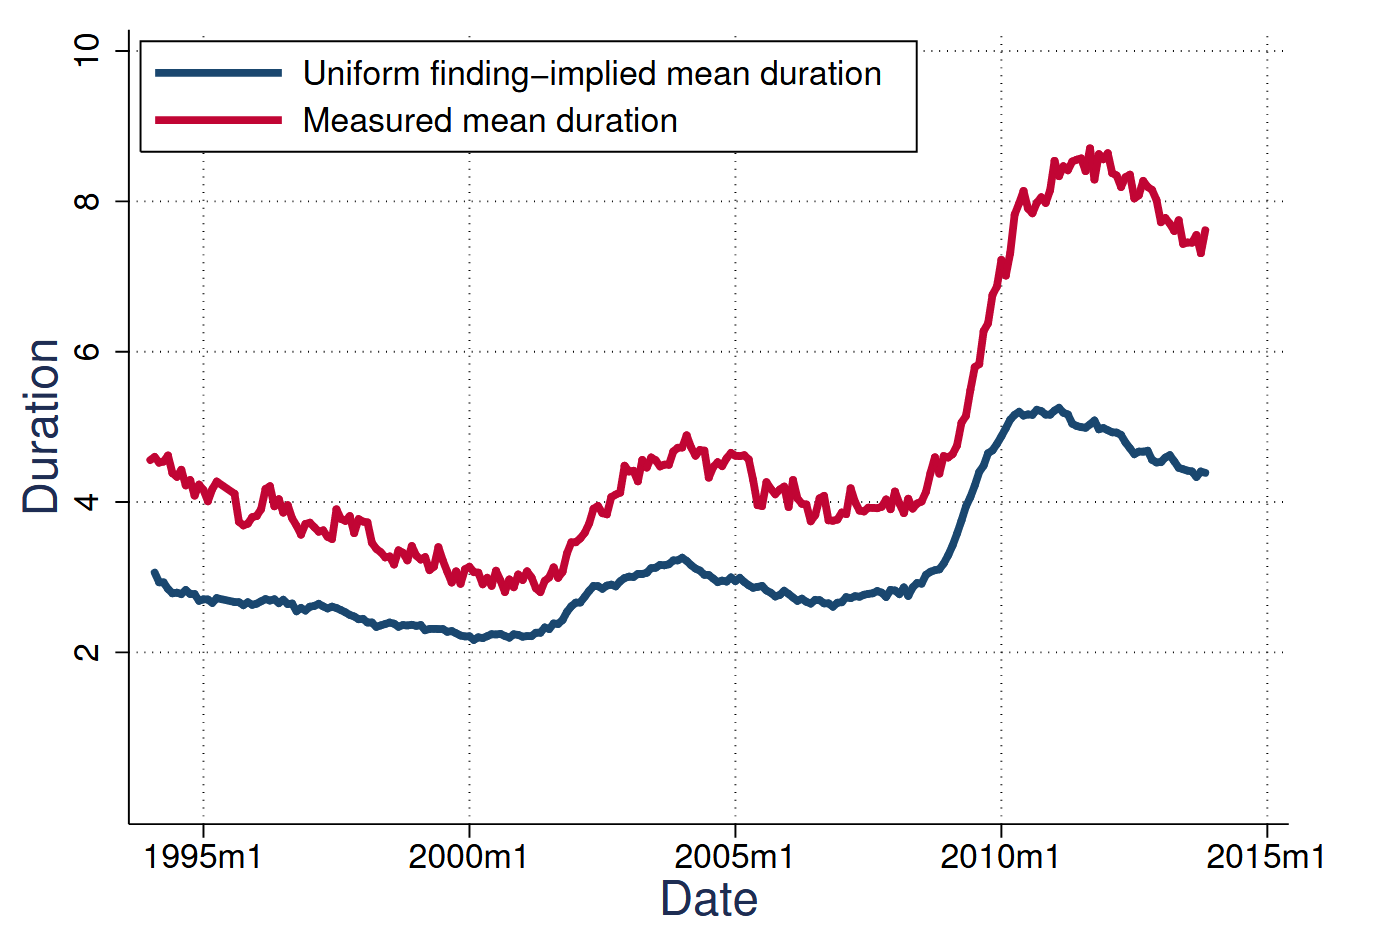
\includegraphics{wiczerLongTermUnemploymentAttached2015_fig1.png}}
        \label{wiczerLongTermUnemploymentAttached2015_fig1}
    \end{center}
\end{figure}

\begin{figure}[H]
    \noindent\caption{Long-term Unemployment}
    \begin{center}
        \resizebox{1\textwidth}{!}{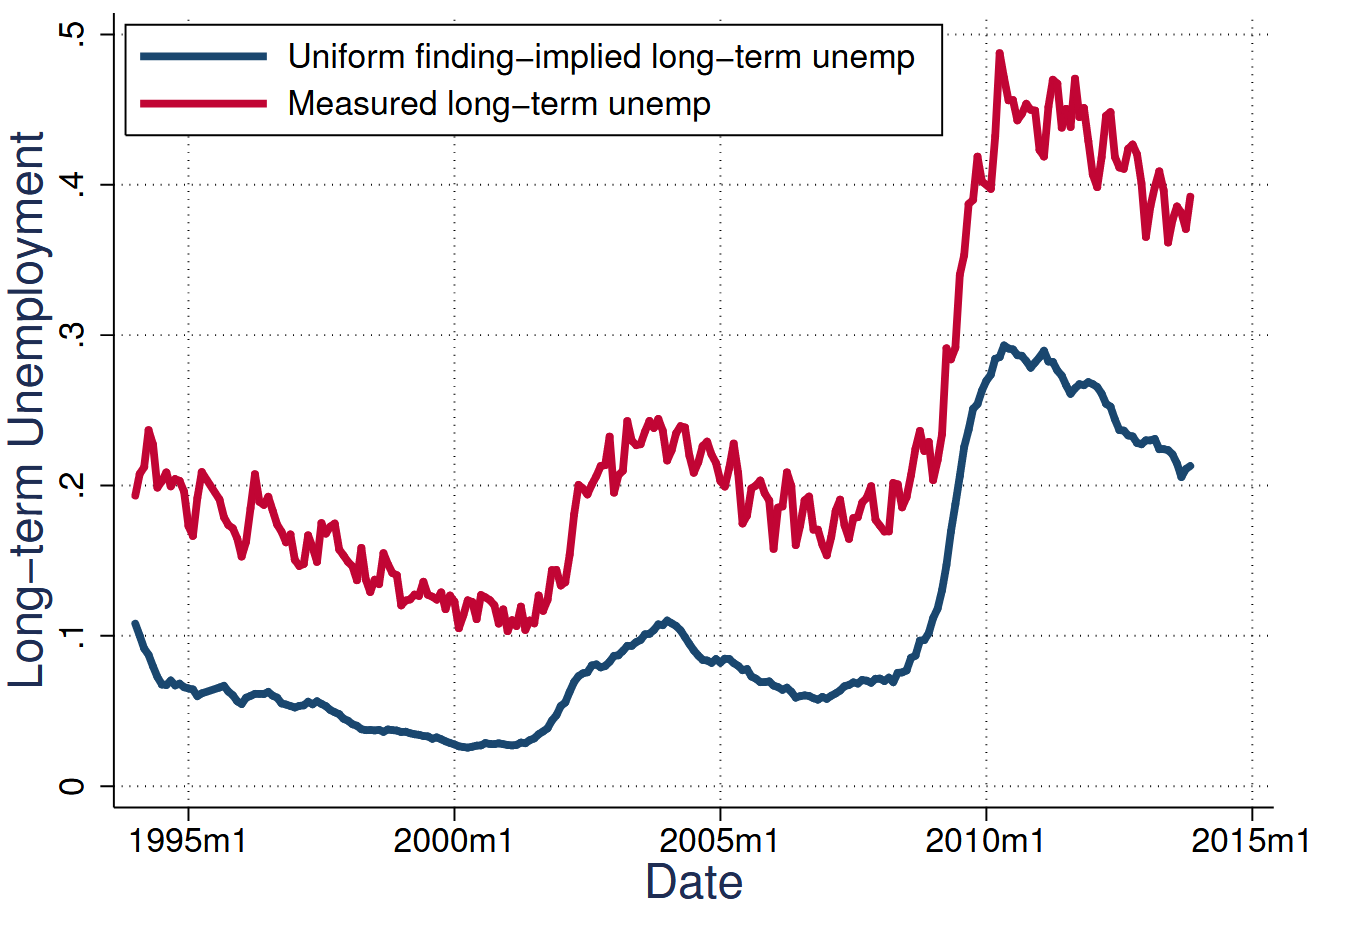
\includegraphics{wiczerLongTermUnemploymentAttached2015_fig2.png}}
        \label{wiczerLongTermUnemploymentAttached2015_fig2}
    \end{center}
\end{figure}

What we are observing in the gap between the statics on unemployment duration and those generated by statistics on job finding is a result of the long-tail of unemployment duration. This is a well-known phenomenon, that the distribution of unemployment duration has a longer tail than the exponential that would be implied by a uniform finding rate. Hence, the average and fraction at long durations are higher than we would observe with a uniform finding rate.

This is statistically and conceptually closely related to duration dependence, in which workers at longer unemployment durations have a lower observed probability of transitioning into employment and this pushes more workers into long unemployment durations, lengthening the distribution's tail. \highlightP{Thus, when we look for factors that will skew upwards the distribution of unemployment duration, we would also be looking for how it affects the relationship between finding rate and unemployment duration.}

\begin{figure}[H]
    \noindent\caption{The job finding rate normalized to the average rate at zero months duration}
    \begin{center}
        \resizebox{1\textwidth}{!}{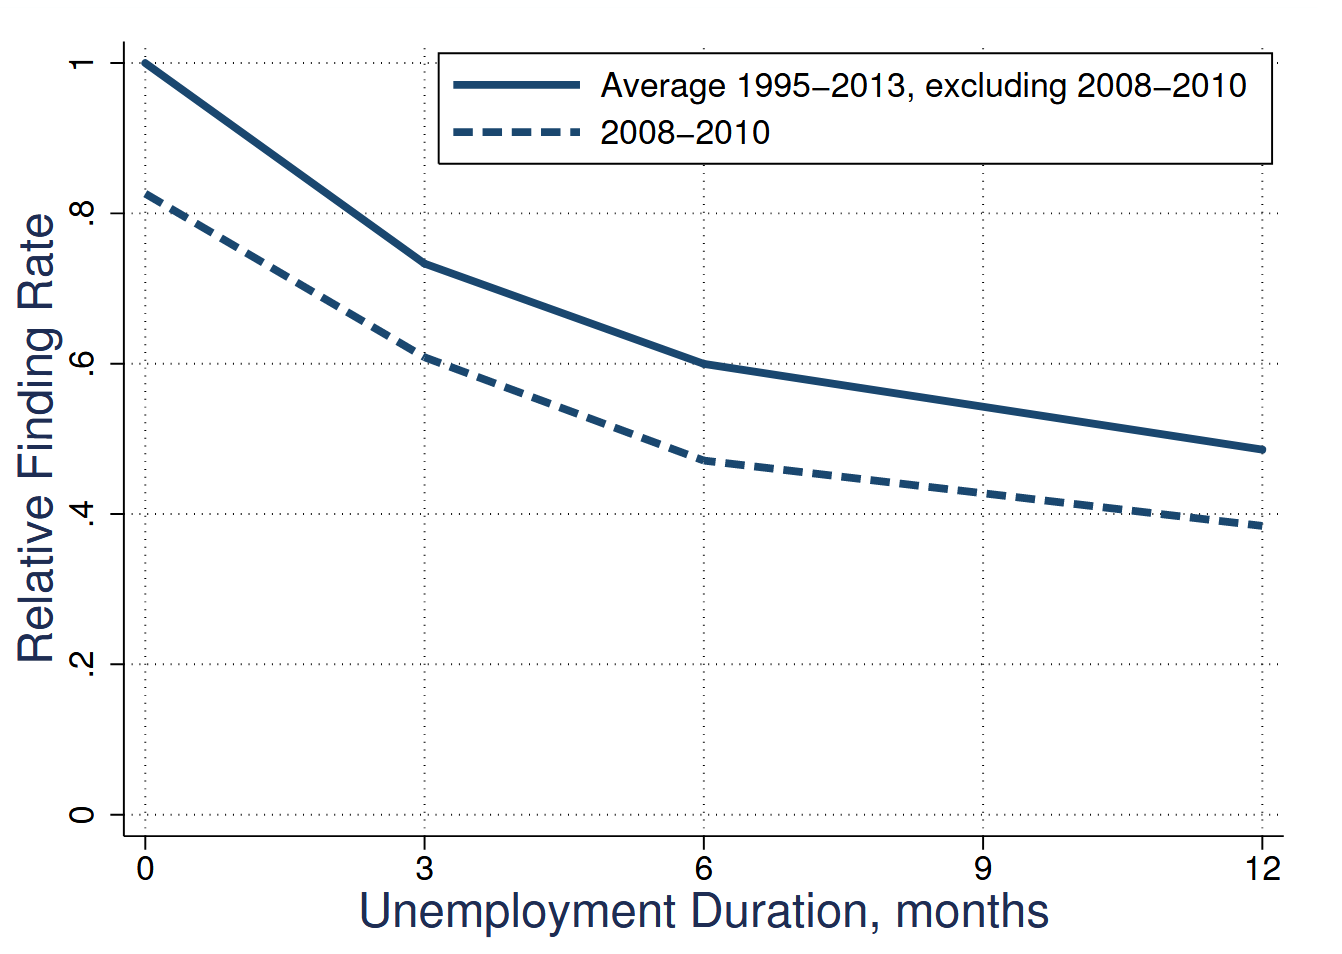
\includegraphics{wiczerLongTermUnemploymentAttached2015_fig3.png}}
        \label{wiczerLongTermUnemploymentAttached2015_fig3}
    \end{center}
\end{figure}

In Figure \ref{wiczerLongTermUnemploymentAttached2015_fig3}, I plot the change in the monthly finding rate at various unemployment durations in my data sample which shows that indeed the rate is declining. I will use this as a consistency check later with results from the model. The literature on duration dependence cites two potential sources of this slope: composition or treatment. The composition effect is that if different types of workers find jobs at different rates, then their composition will change with duration and gradually shift to more slow job finders. The treatment effect is that being unemployed for longer reduces the worker's ability to find a job. In this papery, duration dependence is exclusively due to composition, though only some of the differences are observable, as we will explain below.

\subsection{Heterogeneity Across Occupations}

This paper will link the apparent heterogeneity in finding rates to differences in prior occupation. Once I introduce the structural model, we will see why simple statistical models that condition on past occupation are insufficient, but this section is meant to introduce some of the ideas. I will focus especially on the way that this heterogeneity interacts with business cycles. While other studies attribute differences in finding rate to inherent and unobservable heterogeneity, the connection that I make to prior occupation has several advantages. Most importantly, my tactic imposes additional structural by measuring the observably different incentives that guide agents' choices. \highlightP{If observed dispersion in finding rate is due to attachment to one's prior occupation, then this heterogeneity cannot be summarized by some arbitrary factors that are assumed to be policy neutral.} Moreover, unemployment duration evolves quite differently in different cycles. With a more structural interpretation, we can understand what conditions affect this. In particular, I highlight how duration will increase if occupation-specific skills become more important or there is some mismatch between highly productive occupations and the skills of the unemployed. 

Why is prior occupation a good dimension on which to separate people? A good deal of scholarship has been devoted to the importance of occupation-specific experience and skills. \citet{kambourovOccupationalSpecificityHuman2009} very influentially highlights the returns to occupational tenure as being larger than other forms of tenure, such as employer or industry tenure. In their baseline, they attribute to occupational tenure a 5-year return between $12-20\%$, results  which were amended by Sullivan (2010) but which reconfirmed the overall importance of occupation specific skills. If specific skills are important for wage growth, then potentially they are also important to a worker's experience in unemployment.

Job finding rates and duration are observably different depending on one's prior occupation. From now on, I use the two-digit standard occupational classification (SOC) definition of occupations and make these consistent using the cross-walks provided by Flood et al.  (2015). As can be seen in Figures \ref{wiczerLongTermUnemploymentAttached2015_fig4} and \ref{wiczerLongTermUnemploymentAttached2015_fig5}, the exit from unemployment differs substantially and counter-cyclically across occupations. In Figure \ref{wiczerLongTermUnemploymentAttached2015_fig4}, I show the dispersion in finding rate across occupations, I present this in logs because, as suggested by Elsby et al. (2009), percentage fluctuations are actually more informative than levels about their impact on labor flows. In Figure \ref{wiczerLongTermUnemploymentAttached2015_fig5} I plot the differences in unemployment duration across occupations. Again this dispersion is countercyclical.



\begin{figure}[H]
    \noindent\caption{The variation in finding rate across occupations}
    \begin{center}
        \resizebox{1\textwidth}{!}{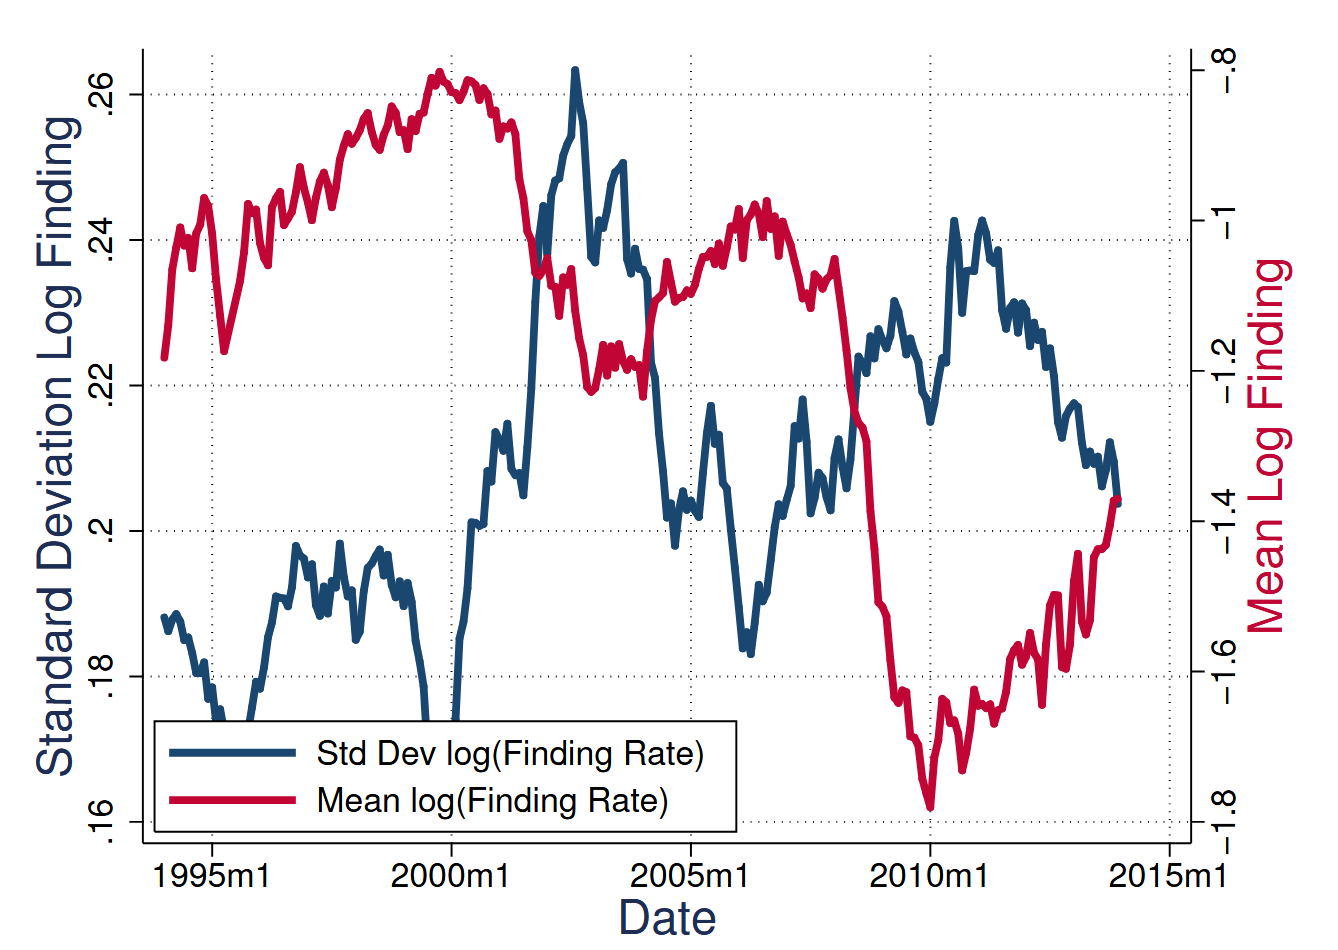
\includegraphics{wiczerLongTermUnemploymentAttached2015_fig4.png}}
        \label{wiczerLongTermUnemploymentAttached2015_fig4}
    \end{center}
\end{figure}

\begin{figure}[H]
    \noindent\caption{The variation in unemployment duration across occupations}
    \begin{center}
        \resizebox{1\textwidth}{!}{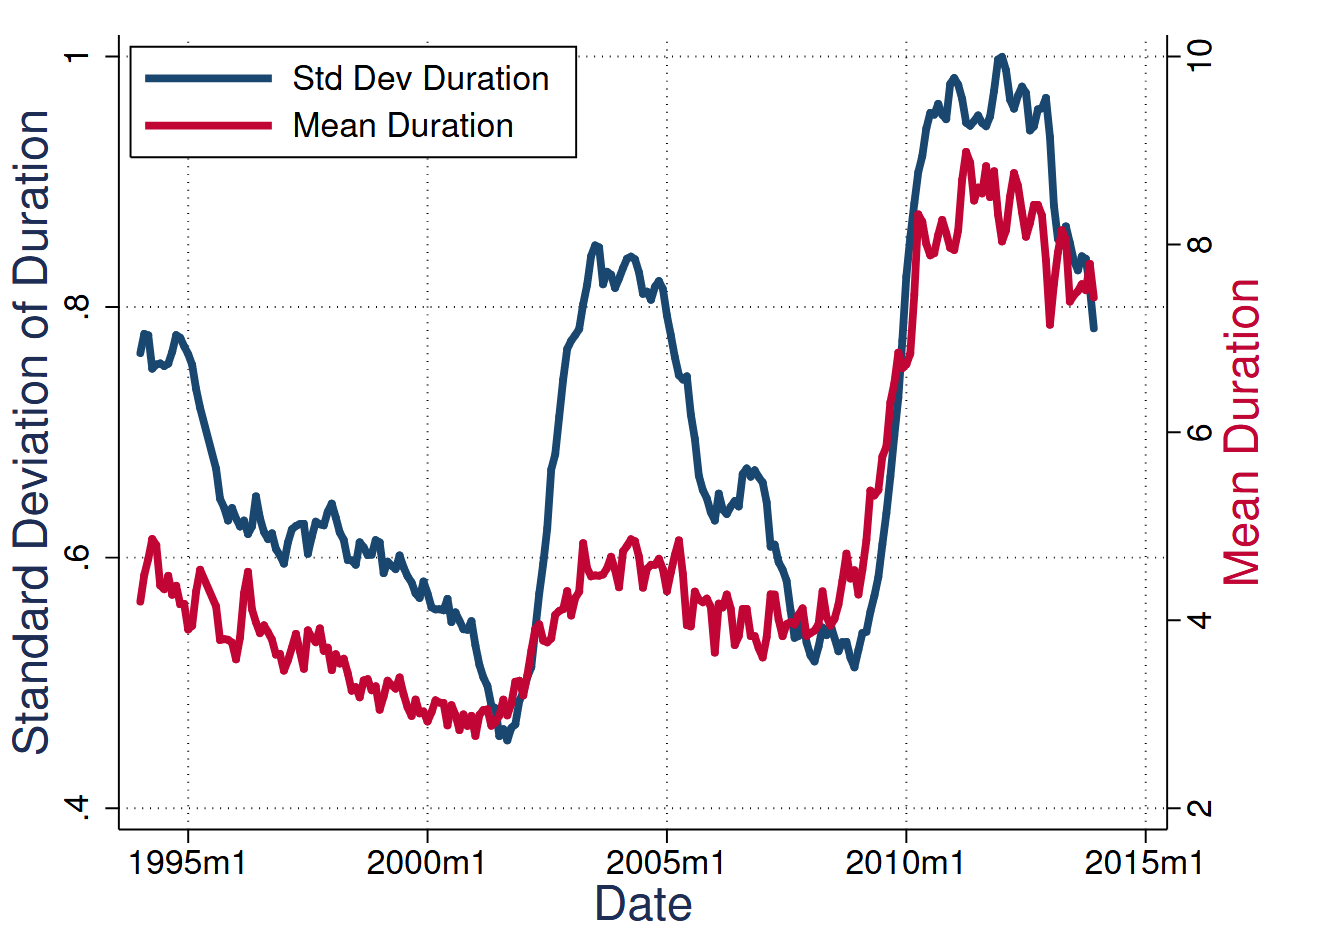
\includegraphics{wiczerLongTermUnemploymentAttached2015_fig5.png}}
        \label{wiczerLongTermUnemploymentAttached2015_fig5}
    \end{center}
\end{figure}

How much of the tail in unemployment duration can be explained purely by occupationlevel heterogeneity? Figure \ref{wiczerLongTermUnemploymentAttached2015_fig6} takes the mean finding rate within a given occupation and then computes the implied unemployment duration. Notice that it is indeed higher than if there were a uniform finding rate, but only barely. In this exercise, we have taken occupations as fixed entities, with the same workers leaving and entering employment. Because these occupations have different flow rates, some longer than others, it does introduce some heterogeneity in the finding rate and hence a tail to unemployment duration that is longer than the exponential implied a uniform finding rate. However, the effect is fairly small, and duration only rises moderately. With occupation-specific finding rates, the average duration is $3.32$ months instead of $3.18$ months with a perfectly equal finding rate across occupations. Both are significantly lower than the time-series average of $4.78$ months in our sample of the data.

\begin{figure}[H]
    \noindent\caption{The variation in unemployment duration across occupations}
    \begin{center}
        \resizebox{1\textwidth}{!}{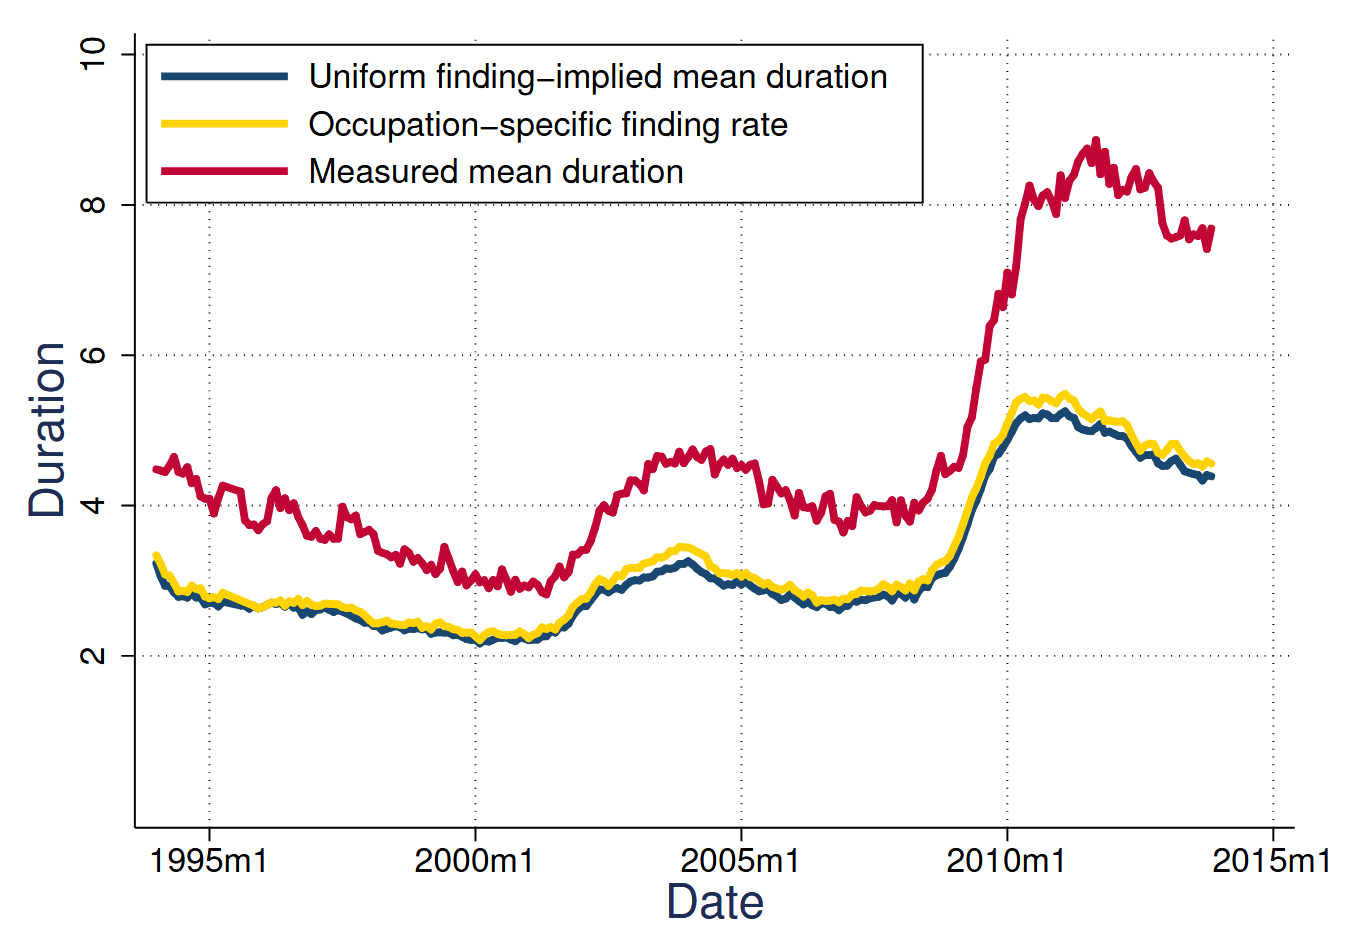
\includegraphics{wiczerLongTermUnemploymentAttached2015_fig6.png}}
        \label{wiczerLongTermUnemploymentAttached2015_fig6}
    \end{center}
\end{figure}

Taking the mean finding rate within an occupation misses much of the heterogeneity. But, it still incorporates the downward slope because some occupations have, on average, slower finding rates. In this exercise we are, however, ignoring the endogenous reallocation across occupations that also may occur among unemployed workers. On average, about half of unemployed workers will match in another occupation. A worker who switches occupations, however, does not simply find a job at the rate of this other occupation, instead they generally have longer unemployment durations.

There is evidently additional heterogeneity among searchers that leads some to find a job in their same occupations and others to switch. Those who switch lose their occupation-specific human capital, and potentially face an entirely different finding rate compared to others who originate in the same occupation. Moreover, switchers do not necessarily go to the occupation with the highest finding rate, depending on a number of factors. In what follows, the model will try to incorporate this additional heterogeneity and the ability to switch occupations.

\section{The Model}

I will present a model of directed search, where the search markets are occupations. Occupations experience productivity shocks and moving across occupations incurs a cost. The model is designed such that parameters can be calibrated and so that the costs of moving across occupations and the process for occupation-specific shocks can both be tied directly to data.

\subsection{Technology and Preferences}

Time is discrete. Production is split into $J$ occupation, and workers have skills suited for various occupations. New workers coming from occupation $\ell$ provide $\o_{\ell d}$ in destination occupation $d$. Here $\o_{\ell\ell}=1$ and $\o_{\ell d}$ will be determined by the data, potentially greater than or less than $1$. Labor in an occupation is aggregated linearly in each type. So if $x_{\ell d}$ is the measure of workers working in $d$ who last worked in $\ell$ then the productive labor force of $d$ is $L_d^{\prime} = \sum_{\ell=0}^{J} \o_{\ell d} x_{\ell d}^{\prime}$. Note that production is done by the labor force at the end of the period after all transitions have completed; hence, it uses $L_d^{\prime}$ rather than Ld that came into the period.

Buffeting these occupations are idiosyncratic shocks $z_d$, which are affected by the average level of productivity, $Z$, and a set of factors $\bds{f}_t$ that are unobservable but help determine comovements. Aggregate productivity follows a simple AR(1) process and the vector of  factors follows a VAR. Productivity shocks are described by the system
\begin{equation}
    \label{wiczerLongTermUnemploymentAttached2015_eq1}
    Z_t = \rho_Z Z_{t-1} + \e_t
\end{equation}
\begin{equation}
    \label{wiczerLongTermUnemploymentAttached2015_eq2}
    z_{d, t} = \l_{f, d} \bds{f}_t + \l_{Z, d} Z_t + \rho_z z_{d, t-1} + \bp{1 - \rho_z} + \zeta_{d, t}
\end{equation}
\begin{equation}
    \label{wiczerLongTermUnemploymentAttached2015_eq3}
    \bds{f}_t = \G \bds{f}_{t-1} + \eta_t
\end{equation}
For future notation, it will be helpful to define $\Zc$ as the state of the joint $Z, \bds{f}, \bc{z_d}$ process. The dispersion in coefficients $\l_{Z, d}$ model differences in cyclical sensitivity, while the factors $\bds{f}_t$ and loadings $\l_{f, d}$ allow for comovements among some occupations beyond their relationship through the aggregate cycle. The form is meant to be parsimonious because there are $J$ occupations and so an estimate for $\E\bs{\zeta \zeta^{\top}}$ is infeasible. 

Several additional shocks govern the effects of worker transitions. Workers become experienced at rate $\tau$, meaning they provide productivity $\o_{dd}=1$. If experienced workers separate, they can keep that experience if they match with the same occupation. Those who are separated while inexperienced become unattached to any occupation, and upon matching with occupation $d$ will provide $\o_{0d}$.

To model endogenous separations, workers who enter the period with a job draw disutility from work $\xi_i \sim H$ which, if it is large enough, will provode a separation. The separation policy will have a cutoff property, so for each $\bp{\ell, d}$ type there will exist $\ol{\xi}$ such that for $\xi < \ol{\xi}$ the match is no longer profitable the separation probability is $s = H\of{\ol{\xi}}$. These shocks are iid, who show that persistence of these shocks is not necessary to match dynamics of separations. By modelling separation-inducing shocks as preferences rather than productivity shocks, I deviate from den Haan et al. (2000) and most of the earlier literature. The problem is that productivity shocks complicate the task of matching observed productivity fluctuations. With productivity shocks, there is ``cleansing'' over the cycles meaning that the primitive shocks are more volatile than those observed. 

When they are searching for a job, there is also another shock $\p \sim F$ that captures their love of the new job. At the beginning of the first period of unemployment, the agent $i$ sees shocks from each occupation he may choose, $\bc{\p_{i,j}}_{j = 1}^{J}$, but only experiences $\p_{i,d}$ in his destination occupation if he successfully finds a job. \highlightP{This preference shock is crucial as it drives gross flows that are far larger than net flows. Its implication is that workers with observably similar characteristics, namely the same occupational work history, have different job finding rates.}

Agents utility is linear and they enjoy consumption on top of the shocks. To summarize, worker $i$ who stays matched the entire period will experience flow utility $c_i + \xi_i$. If that worker was newly matched in occupation $d$ in that period he experiences $c_i + \p_{i,d}$.

\subsection{Unemployment Benefits}

Workers who are unemployed receive a flow utility $b_i$. If they are still eligible for benefits, $e = 1$, this is a $40\%$ replacement of their former salary. With probability $\d$ benefits expire, $e = 0$, and then they receive food stamp support, as in Nakajima (2012), at about $17\%$ of average earnings. \highlightP{This random expiration saves unemployment duration from becoming a state.} I denote $\d$ here as a parameter, but in reality it actually fluctuates over the cycle.

Note that unemployed workers do not enjoy leisure utility, which Hagedorn and Manovskii (2008) and others have shown plays an important role in matching the volatility of vacancy postings. This is because those working experience disutility from work and that plays a  similar role in reducing the expected surplus from a match.

\subsection{Search and Market Structure}















\bibliography{\CiteReference} 

\end{document}